\documentclass[11pt,a4paper]{article}
\usepackage[slovene]{babel}
\usepackage[utf8]{inputenc}
\usepackage[T1]{fontenc}
\usepackage{amsmath,amssymb}
\usepackage{graphicx}
\usepackage{booktabs}
\usepackage[margin=2.5cm]{geometry}

\title{Točka 1: dve točki v treh dimenzijah}
\author{Ana Poklukar}
\date{\today}

\begin{document}
\maketitle

\section{Vprašanje}

Dani sta dve točki v kocki $[0,1]^3$ in v vsaki predpisana vrednost. Ali obstaja kopula, ki ima v teh dveh točkah ravno predpisani vrednosti? De Baets in soavtorji~\cite{DeBaets} so pokazali, da vedno. Tu isti rezultat dobimo z metodo iz članka~\cite{OVZ}, v obliki s sestanka 28.~9.

Do zamenjave točk in vrstnega reda koordinat sta možni dve konfiguraciji: v konfiguraciji $3+0$ je ena točka večja od druge v vseh treh koordinatah, v konfiguraciji $2+1$ pa je v dveh koordinatah večja in v eni manjša. Vsako obravnavamo posebej.

\section{Določene in nedoločene vrednosti}

Kocko razrežemo pri koordinatah obeh točk. Po vsaki osi dobimo štiri vrednosti ($0$, manjša, večja, $1$), torej $64$ vozlišč in $27$ celic. Neznanke so vrednosti kopule v vozliščih.

Veliko vrednosti je znanih vnaprej:
\begin{itemize}
    \item če je katera koordinata enaka $0$, je vrednost $0$;
    \item če so vse koordinate razen ene enake $1$, je vrednost enaka tej koordinati;
    \item v obeh točkah je vrednost predpisana.
\end{itemize}
To so \emph{določena} vozlišča, v treh dimenzijah jih je $46$. Ostalih $18$ je \emph{nedoločenih}, v obeh konfiguracijah (slika~\ref{fig:vozlisca}).

\begin{figure}[ht]
\centering
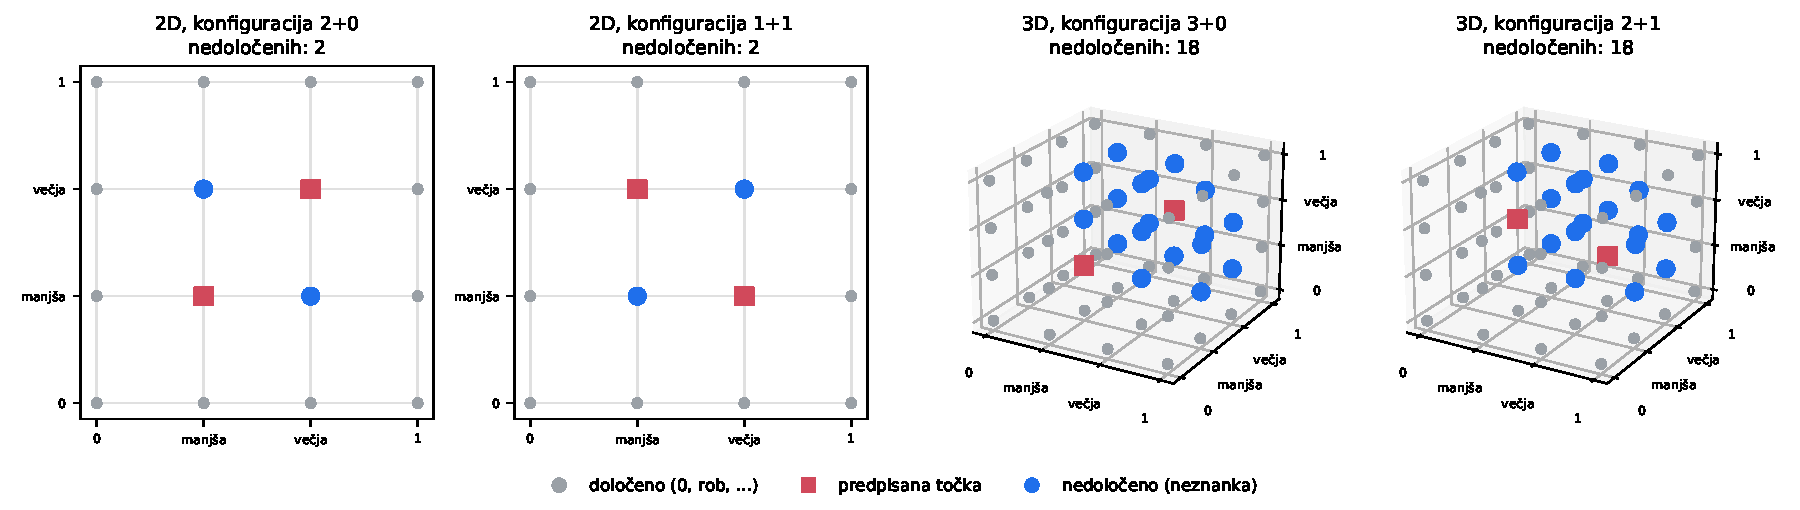
\includegraphics[width=\textwidth]{../slike/slika_vozlisca.pdf}
\caption{Določena vozlišča (sivo), predpisani točki (rdeče) in nedoločena vozlišča (modro).}
\label{fig:vozlisca}
\end{figure}

\section{Sistem neenačb}

Naj bo $H$ incidenčna matrika velikosti $27 \times 64$, tako da je $(Hv)_B$ volumen celice $B$. Po izreku~4.4 v~\cite{OVZ} kopula obstaja natanko tedaj, ko lahko nedoločene vrednosti izberemo tako, da je
\begin{itemize}
    \item volumen vsake celice nenegativen, $Hv \ge 0$,
    \item vsaka nedoločena vrednost med spodnjo in zgornjo ovojnico iz (3.4) in (3.5) v~\cite{OVZ}, $a_n \le v_n \le b_n$.
\end{itemize}
Stolpce matrike $H$ razdelimo na nedoločene in določene, $H = [H_n \mid H_d]$, tako da je $Hv = H_n v_n + H_d v_d$ (slika~\ref{fig:razbitje}). Določeni del prenesemo na desno stran in vse skupaj zapišemo kot en sistem
\[
    G v_n \le h, \qquad
    G = \begin{bmatrix} -H_n \\ I \\ -I \end{bmatrix}, \qquad
    h = \begin{bmatrix} H_d v_d \\ b_n \\ -a_n \end{bmatrix}.
\]
To je sistem (4.17) iz~\cite{OVZ}, le da so določene vrednosti na desni strani. Matrika $G$ je velikosti $63 \times 18$ in je odvisna samo od konfiguracije. Vektor $h$ je odvisen od podatkov, torej od koordinat točk in predpisanih vrednosti.

\begin{figure}[ht]
\centering
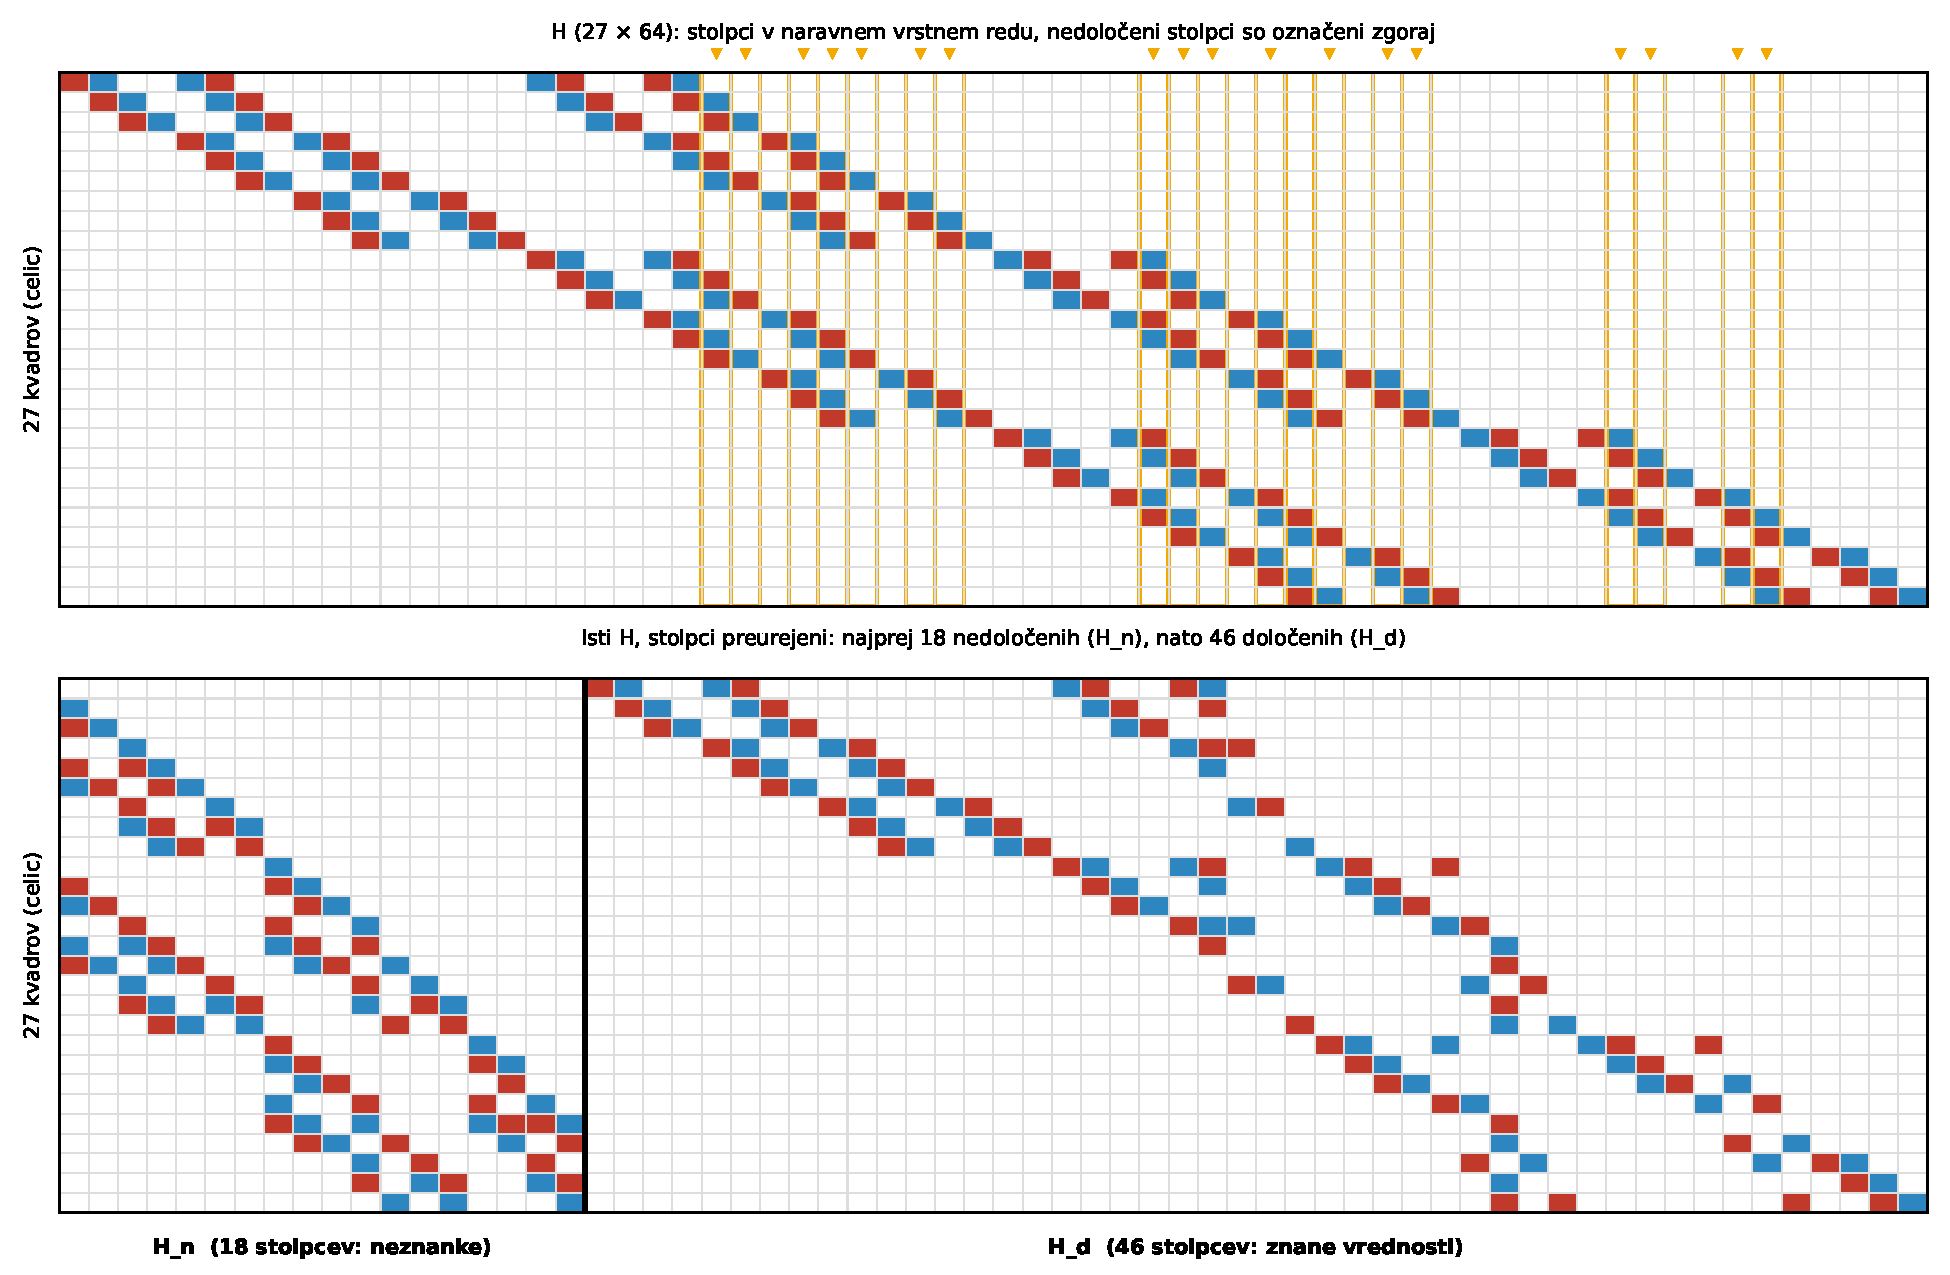
\includegraphics[width=0.85\textwidth]{../slike/slika_razbitje_H.pdf}
\caption{Matrika $H$ (modro $+1$, rdeče $-1$) in njeno razbitje na $H_n$ in $H_d$ v konfiguraciji $3+0$.}
\label{fig:razbitje}
\end{figure}

\section{Dualni problem}

Namesto da iščemo rešitev sistema, iščemo dokaz, da rešitve ni. Po Farkasovi lemi ima sistem $G v_n \le h$ rešitev natanko tedaj, ko za vsak $y \ge 0$ z $G^{\mathsf T} y = 0$ velja $h^{\mathsf T} y \ge 0$.

Vektor $y$ pove, katere neenačbe sistema seštejemo in s kolikšnimi utežmi. Pogoj $G^{\mathsf T} y = 0$ pomeni, da se v vsoti vse neznanke pokrajšajo. Ostane neenakost $h^{\mathsf T} y \ge 0$, v kateri nastopajo samo podatki.

Če $y$ pomnožimo s pozitivnim številom, dobimo isto neenakost, zato lahko privzamemo $y_1 + \dots + y_{63} = 1$. Vsi taki $y$ tvorijo politop $P$, ki je odvisen samo od konfiguracije. Izraz $h^{\mathsf T} y$ je v $y$ linearen, zato je najmanjši v enem od oglišč politopa $P$. Zadošča torej za vsako konfiguracijo enkrat izračunati oglišča politopa $P$ in za vsako preveriti, da je $h^{\mathsf T} y \ge 0$.

Del vektorja $y$, ki pripada celicam, ustreza $\lambda$ iz~\cite{OVZ}, izraz $h^{\mathsf T} y$ pa funkciji $\Phi_E(\lambda)$.

V dveh dimenzijah sta nedoločeni le dve vozlišči in politop $P$ ima $23$ oglišč. Primer oglišča v konfiguraciji $2+0$, kjer ima večja točka $(l_1, l_2)$ vrednost $q_2$, je celica desno zgoraj. Vsa njena vozlišča so določena, njen volumen $1 - l_1 - l_2 + q_2 \ge 0$ pa je ravno spodnja Fréchet--Hoeffdingova meja za $q_2$. Na mreži iz primera~4.1 v~\cite{OVZ} dobimo $21$ oglišč z $\lambda \ne 0$ in vsa so med $159$ oglišči iz primera~4.5.

\section{Rezultati v treh dimenzijah}

Postopek smo implementirali v Pythonu. Oglišča politopa $P$ smo izračunali s knjižnico cdd~\cite{cdd} in za vsako točno preverili, da velja $y \ge 0$ in $G^{\mathsf T} y = 0$.

\begin{center}
\begin{tabular}{lcc}
\toprule
 & $3+0$ & $2+1$ \\
\midrule
nedoločena vozlišča & $18$ & $18$ \\
velikost matrike $G$ & $63 \times 18$ & $63 \times 18$ \\
oglišča politopa $P$ & $26\,966$ & $32\,224$ \\
oglišča do zamenjave koordinat & $4\,812$ & $16\,460$ \\
čas izračuna oglišč & manj kot minuta & manj kot minuta \\
\bottomrule
\end{tabular}
\end{center}

Da v seznamu nobeno oglišče ne manjka, smo preverili z linearnim programom. Za $300$ naključnih naborov podatkov, tudi takih, za katere kopula ne obstaja, se odgovor po ogliščih vedno ujema z odgovorom linearnega programa.

\paragraph{Preverjanje na naključnih podatkih.} Vsako oglišče da neenakost $h^{\mathsf T} y \ge 0$, ki mora veljati za vse združljive podatke. Najprej smo jih preverili na $2000$ naključnih združljivih podatkih za vsako konfiguracijo. Koordinate točk so naključne, vrednosti pa so izbrane naključno znotraj dovoljenega intervala ali na njegovem robu. Nobena neenakost ni bila kršena.

\paragraph{Preverjanje za vse podatke.} Podatki so osem števil: po dve koordinati na vsaki osi in dve predpisani vrednosti. Vsi združljivi podatki ene konfiguracije tvorijo politop, ki ima $27$ oglišč. Zgornja ovojnica $b_s$ je najmanjši od več linearnih izrazov v podatkih, spodnja ovojnica $a_s$ pa največji. V $h^{\mathsf T} y$ nastopa $b_s$ s plusom in $a_s$ z minusom, zato je $h^{\mathsf T} y$ najmanjši od več linearnih izrazov. Vsak linearen izraz je na politopu najmanjši v enem od oglišč, zato zadošča neenakosti preveriti v $27$ ogliščih politopa podatkov. To smo naredili točno, z ulomki: vse neenakosti veljajo v vseh $27$ ogliščih, v obeh konfiguracijah. Ta argument je nastal s pomočjo orodja umetne inteligence.

Za dve točki v treh dimenzijah torej kopula vedno obstaja, kar se ujema z rezultatom iz~\cite{DeBaets}.

\paragraph{Primerjava.} Dokaz v~\cite{DeBaets} poteka z ročno izbranimi pivotnimi koraki, ločenimi glede na predznake več izrazov. Tu je postopek mehaničen in za eno konfiguracijo traja nekaj minut, oglišč pa je preveč, da bi jih pregledali ročno.

\begin{thebibliography}{9}
\raggedright
\bibitem{DeBaets}
B.~De Baets, H.~De Meyer, J.~Fernández-Sánchez, M.~Úbeda-Flores,
\emph{On the existence of a trivariate copula with given values of a trivariate quasi-copula at several points},
Fuzzy Sets and Systems \textbf{228} (2013) 3--14.

\bibitem{cdd}
K.~Fukuda, \emph{cddlib}, \texttt{https://github.com/cddlib/cddlib}. Uporabljeno prek paketa pycddlib.

\bibitem{OVZ}
M.~Omladič, M.~Vuk, A.~Zalar,
\emph{A linear programming approach to finite copula interpolation}, rokopis.
\end{thebibliography}

\end{document}
